% execution-graph-iff.tex
\documentclass[tikz,border=6pt]{standalone}
\usepackage{xcolor}
\usetikzlibrary{arrows.meta,positioning}

\definecolor{Navy}{RGB}{20,54,92}
\definecolor{Teal}{RGB}{17,119,125}
\definecolor{Accent}{RGB}{184,63,49}
\newcommand{\Histo}{\mathcal{H}}
\newcommand{\Exec}{\mathcal{A}}
\newcommand{\Graph}{\mathcal{G}}
\newcommand{\VIS}{\mathsf{VIS}}
\newcommand{\AR}{\mathsf{AR}}
\newcommand{\SO}{\mathsf{SO}}
\newcommand{\WR}{\mathsf{WR}}
\newcommand{\WW}{\mathsf{WW}}
\newcommand{\RW}{\mathsf{RW}}
\newcommand{\PredWR}{\mathsf{PredWR}}
\newcommand{\PredRW}{\mathsf{PredRW}}

\begin{document}
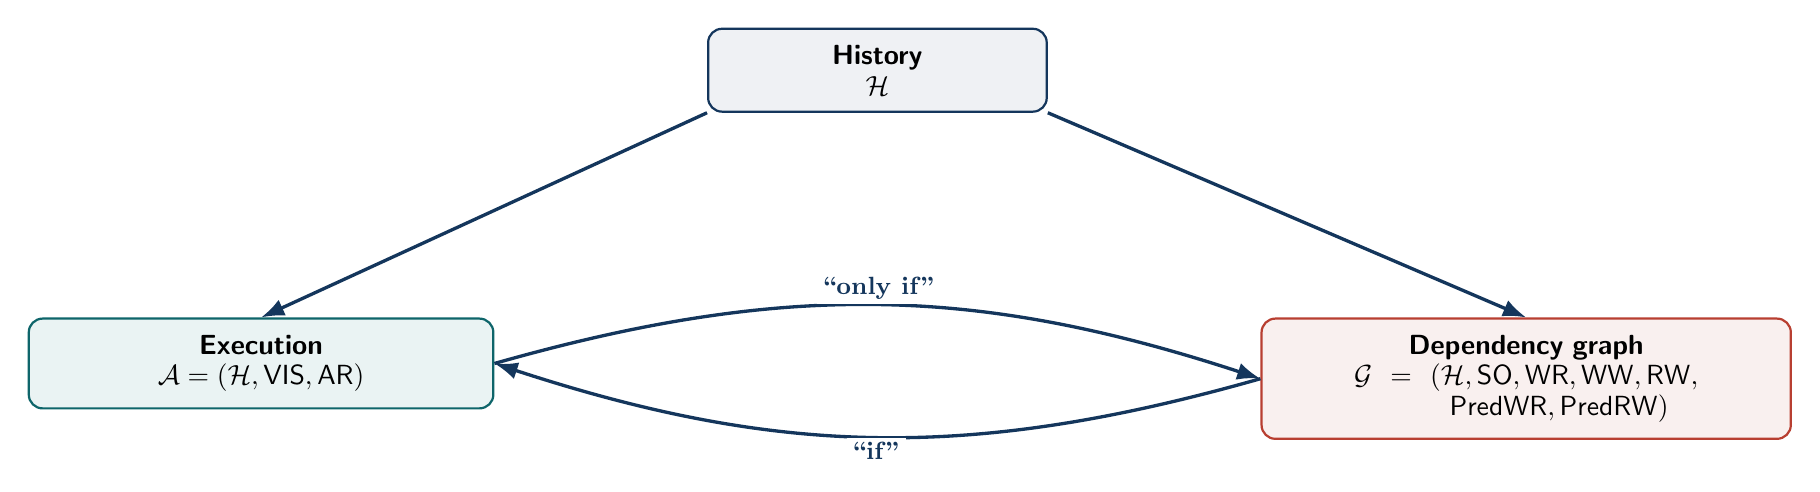
\begin{tikzpicture}[
  font=\sffamily,
  >=Latex,
  node distance=26mm and 27mm,
  witness/.style={rounded corners=5pt, thick, align=center, inner sep=6pt},
  history/.style={witness, draw=Navy, fill=Navy!7, minimum width=43mm},
  execution/.style={witness, draw=Teal!85!black, fill=Teal!9, minimum width=59mm},
  graph/.style={witness, draw=Accent, fill=Accent!8, text width=63mm},
  construction/.style={-Latex, very thick, Navy}
]
  \node[history] (h) {\textbf{History}\\[-1pt]$\Histo$};
  \node[execution, below left=of h] (a)
    {\textbf{Execution}\\[-1pt]
     $\Exec=(\Histo,\VIS,\AR)$};
  \node[graph, below right=of h] (g)
    {\textbf{Dependency graph}\\[-1pt]
     $\Graph=(\Histo,\SO,\WR,\WW,\RW,$\\[-1pt]
     $\phantom{\Graph=(}\PredWR,\PredRW)$};

  \draw[construction] (h.south west) -- (a.north);
  \draw[construction] (h.south east) -- (g.north);
  \draw[construction, bend left=17] (a.east) to
    node[above, font=\bfseries\small, fill=white, inner sep=1.5pt] {``only if''} (g.west);
  \draw[construction, bend left=17] (g.west) to
    node[below, font=\bfseries\small, fill=white, inner sep=1.5pt] {``if''} (a.east);
\end{tikzpicture}
\end{document}
